\documentclass{beamer}
\usepackage[utf8]{inputenc}
\usepackage{graphicx}
\usepackage{amsmath}
\usepackage{tikz}
\usetikzlibrary{positioning, shapes, arrows, er, decorations.pathmorphing, backgrounds, fit, petri}

% Tema della presentazione
\usetheme{Madrid}
\usecolortheme{default}

% Informazioni del documento
\title{La progettazione delle basi di dati}
\subtitle{Progettazione Concettuale}
\author{Prof. Fedeli Massimo}
\institute{IIS Fermi Sacconi Ceci - Ascoli Piceno}
\date{\today}

\begin{document}
	
	% Slide titolo
	\begin{frame}
		\titlepage
	\end{frame}
	
	% Slide 1: La progettazione del database
	\begin{frame}{La progettazione del database}
		I passi principali per progettare un database si possono così schematizzare:
		\begin{enumerate}
			\item Analisi del problema
			\item Progettazione concettuale del database $\rightarrow$ modello E-R
			\item Progettazione logica del database $\rightarrow$ schema logico
			\item Progettazione fisica e implementazione
			\item Realizzazione delle applicazioni $\rightarrow$ (Java, VB, PHP, etc)
		\end{enumerate}
		
		\vspace{0.3cm}
		Ognuno di questi passi presenta delle criticità e implica un insieme di operazioni anche complesse tra cui:
		\begin{itemize}
			\item la fase di sviluppo del database
			\item la fase di sviluppo dell'applicazione
			\item i test di funzionamento di entrambi, il collaudo ecc
		\end{itemize}
	\end{frame}
	
	% Slide 2: Le fasi della progettazione
	\begin{frame}{Le fasi della progettazione di un database}
		\begin{center}
			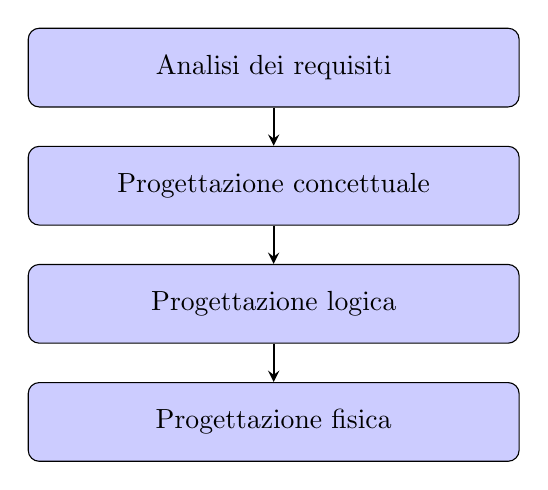
\begin{tikzpicture}[node distance=1.5cm, auto]
				\tikzstyle{box} = [rectangle, draw, fill=blue!20, text width=6cm, text centered, rounded corners, minimum height=1cm]
				\tikzstyle{arrow} = [thick,->,>=stealth]
				
				\node [box] (analisi) {Analisi dei requisiti};
				\node [box, below of=analisi] (concettuale) {Progettazione concettuale};
				\node [box, below of=concettuale] (logica) {Progettazione logica};
				\node [box, below of=logica] (fisica) {Progettazione fisica};
				
				\draw [arrow] (analisi) -- (concettuale);
				\draw [arrow] (concettuale) -- (logica);
				\draw [arrow] (logica) -- (fisica);
			\end{tikzpicture}
		\end{center}
		
		\vspace{0.3cm}
		L'output della progettazione concettuale è il \textbf{modello concettuale}.
	\end{frame}
	
	% Slide 3: I livelli di astrazione
	\begin{frame}{I livelli di astrazione del modello di database}
		\begin{columns}
			\column{0.5\textwidth}
			La progettazione di un modello di dati avviene a diversi livelli di astrazione:
			
			\begin{itemize}
				\item \textbf{Livello concettuale}
				\item \textbf{Livello logico}
				\item \textbf{Livello fisico}
			\end{itemize}
			
			\column{0.5\textwidth}
			\begin{center}
				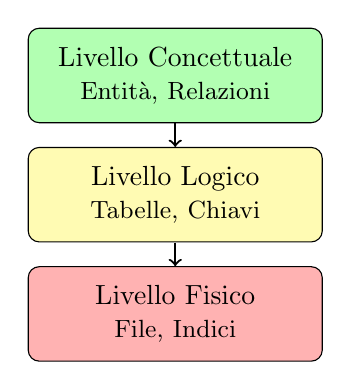
\begin{tikzpicture}[scale=0.8]
					\tikzstyle{level} = [rectangle, draw, fill=blue!20, text width=3.5cm, text centered, rounded corners, minimum height=1.2cm]
					
					\node [level, fill=green!30] (concettuale) {Livello Concettuale\\{\small Entità, Relazioni}};
					\node [level, fill=yellow!30, below=0.3cm of concettuale] (logico) {Livello Logico\\{\small Tabelle, Chiavi}};
					\node [level, fill=red!30, below=0.3cm of logico] (fisico) {Livello Fisico\\{\small File, Indici}};
					
					\draw [->, thick] (concettuale) -- (logico);
					\draw [->, thick] (logico) -- (fisico);
				\end{tikzpicture}
			\end{center}
		\end{columns}
		
		\vspace{0.3cm}
		\small Il livello fisico è l'implementazione del livello logico sui supporti per la registrazione fisica dei dati (partizioni, puntatori, blocchi fisici, cluster, indici).
	\end{frame}
	
	% Slide 4: Analisi preliminare
	\begin{frame}{Analisi preliminare alla modellazione}
		L'analisi preliminare per la modellazione dei dati avviene solitamente cercando di individuare:
		\begin{itemize}
			\item le esigenze del cliente
			\item il dominio dell'applicazione
			\item quali informazioni devono essere salvate
			\item in che modo queste informazioni verranno manipolate dall'utente
		\end{itemize}
		
		\vspace{0.5cm}
		Le tecniche di analisi del problema sono da considerarsi valide e applicabili anche alla progettazione dei database: naturalmente bisognerà prestare maggiore attenzione al dato e quindi spesso la tecnica \textbf{bottom-up} è da preferirsi a quella top-down.
	\end{frame}
	
	% Slide 5: La fase di modellazione
	\begin{frame}{La fase di modellazione}
		Al termine dell'analisi inizia la prima fase di modellazione, che è quella concettuale; per attuarla, si può far ricorso ai due seguenti modelli:
		\begin{itemize}
			\item modello entità-relazione
			\item modello a oggetti
		\end{itemize}
		
		\vspace{0.5cm}
		Benché il secondo modello stia cominciando a rivelarsi interessante da un punto di vista commerciale e non solamente accademico, la stragrande maggioranza delle applicazioni esistenti ricorre all'approccio \textbf{Entità-Relazione (E-R)}.
	\end{frame}
	
	% Slide 6: Modello E-R
	\begin{frame}{Modello entità-relazione}
		\begin{columns}
			\column{0.5\textwidth}
			Il modello Entità-Relazione consente di superare questo ostacolo in quanto è assolutamente indipendente dal linguaggio scritto o parlato e permette quindi a tutti di comprendere la struttura del database.
			
			\vspace{0.3cm}
			Di norma, al modello Entità-Relazione viene affiancato un \textbf{documento tecnico} che descrive in maggior dettaglio i concetti espressi graficamente.
			
			\column{0.5\textwidth}
			\begin{center}
				\textbf{Simboli principali}
				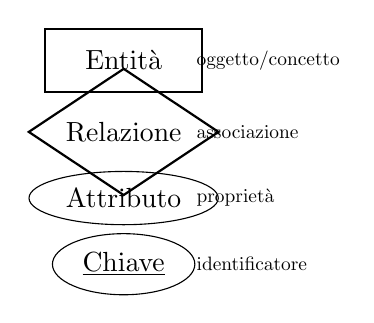
\begin{tikzpicture}[scale=0.7]
					% Entità
					\node[rectangle, draw, thick, minimum width=2cm, minimum height=0.8cm] at (0,0) {Entità};
					\node[right, scale=0.7] at (1.2,0) {oggetto/concetto};
					
					% Relazione
					\node[diamond, draw, thick, minimum width=1.2cm, aspect=1.5] at (0,-1.3) {Relazione};
					\node[right, scale=0.7] at (1.2,-1.3) {associazione};
					
					% Attributo
					\node[ellipse, draw] at (0,-2.5) {Attributo};
					\node[right, scale=0.7] at (1.2,-2.5) {proprietà};
					
					% Chiave primaria
					\node[ellipse, draw] at (0,-3.7) {\underline{Chiave}};
					\node[right, scale=0.7] at (1.2,-3.7) {identificatore};
				\end{tikzpicture}
			\end{center}
		\end{columns}
	\end{frame}
	
	% Slide 7: Scopi del modello E-R
	\begin{frame}{Progettazione concettuale $\rightarrow$ modello entità-relazione}
		\begin{itemize}
			\item Il primo scopo del modello Entità-Relazione è quello di fornire la \textbf{rappresentazione grafica} di tutti gli oggetti che fanno parte di un database così che il flusso delle informazioni possa essere seguito e verificato prima di sviluppare l'applicazione
			
			\vspace{0.3cm}
			\item In secondo luogo, questo modello può essere usato dagli sviluppatori per \textbf{creare il database fisico} e tutti gli oggetti che ne fanno parte
		\end{itemize}
	\end{frame}
	
	% Slide 8: Caratteristiche del modello concettuale
	\begin{frame}{Caratteristiche del modello concettuale}
		\begin{itemize}
			\item \textbf{Correttezza} (Uso corretto degli strumenti): utilizzo appropriato degli strumenti di modellazione concettuale secondo le loro finalità
			
			\item \textbf{Completezza} (Modellazione di tutti gli aspetti rilevanti della realtà): rappresentazione di tutti gli aspetti significativi del dominio applicativo da modellare
			
			\item \textbf{Chiarezza} (Modello leggibile e informazioni comprensibili): facilità di lettura del modello e comprensione delle informazioni rappresentate
			
			\item \textbf{Indipendenza} (Non dipendente dagli strumenti informatici successivi): il modello concettuale non deve dipendere da implementazioni o strumenti informatici specifici
		\end{itemize}
	\end{frame}
	
	% Slide 9: Correttezza
	\begin{frame}{Correttezza}
		Il modello concettuale deve utilizzare gli strumenti di modellazione (come diagrammi ER, UML, BPMN, ecc.) secondo la loro finalità specifica, senza forzature o interpretazioni errate.
		
		\vspace{0.3cm}
		Non si tratta solo di "usare lo strumento": un diagramma ER, ad esempio, serve a rappresentare relazioni tra entità, non flussi di processo. Usarlo per descrivere un workflow sarebbe un errore concettuale.
		
		\vspace{0.3cm}
		\textbf{Coerenza semantica}: Ogni simbolo (es. rombo per le relazioni, rettangoli per le entità) deve rispettare le convenzioni stabilite.
	\end{frame}
	
	% Slide 10: Indipendenza
	\begin{frame}{Indipendenza}
		Il modello concettuale deve essere astratto e neutrale, non vincolato a tecnologie, DBMS o linguaggi di programmazione specifici. Si deve descrivere \textit{cosa fare}, non \textit{come implementarlo}.
		
		\vspace{0.3cm}
		\textbf{Vantaggi:}
		\begin{itemize}
			\item Longevità (il modello sopravvive ai cambi tecnologici)
			\item Flessibilità (può essere implementato in diversi modi)
		\end{itemize}
		
		\vspace{0.3cm}
		\textbf{Esempio pratico:}
		\begin{itemize}
			\item \textcolor{red}{Dipendente}: Scrivere nel modello "Usare PostgreSQL con trigger per gestire cancellazioni"
			\item \textcolor{green}{Indipendente}: Definire una regola di business come "Una prenotazione cancellata deve aggiornare la disponibilità della risorsa", senza menzionare tecnologie
		\end{itemize}
	\end{frame}
	
	% Slide 11: Caratteristiche della progettazione concettuale
	\begin{frame}{Caratteristiche della progettazione concettuale}
		La progettazione concettuale deve essere:
		
		\begin{itemize}
			\item \textbf{Rigorosa} $\rightarrow$ per non lasciare dubbi in merito alle caratteristiche della base di dati che si sta progettando
			
			\item \textbf{Espressa con formalismi semplici} $\rightarrow$ per consentire la lettura e la comprensione anche da parte di utenti non tecnici
		\end{itemize}
		
		\vspace{0.5cm}
		Gli utenti devono infatti essere certi che i progettisti abbiano compreso a fondo tutte le loro esigenze.
		
		\vspace{0.3cm}
		Il modello \textbf{entità/associazioni (relazioni)} ha queste caratteristiche e si concretizza in un documento con schemi grafici.
	\end{frame}
	
	% Slide 12: Il modello concettuale
	\begin{frame}{La progettazione concettuale $\rightarrow$ il modello concettuale}
		\begin{itemize}
			\item Un aspetto rilevante del modello concettuale sono concetti e formalismi utilizzati nella costruzione del modello entità/associazioni
			
			\item Il modello concettuale, pur essendo molto utilizzato nella progettazione concettuale, \textbf{non ha una rappresentazione standardizzata}
			
			\item Il modello entità/associazioni è composto da \textbf{entità}, \textbf{associazioni} e \textbf{attributi} e che cosa si intenda con tali termini: esistono però diversi modi di rappresentarli
			
			\item La notazione classica e la notazione standard UML
		\end{itemize}
	\end{frame}
	
	% Slide 13: Il database designer
	\begin{frame}{Chi realizza il modello concettuale? Il database designer}
		Il \textbf{database designer} è responsabile dell'astrazione dei dati dal mondo reale a partire dall'analisi dei requisiti fino a ottenere la corretta modellazione degli stessi nello schema concettuale e successivamente nello schema logico.
	\end{frame}
	
	% Slide 14: I compiti del database designer
	\begin{frame}{I compiti del database designer}
		\begin{itemize}
			\item Il primo compito di un database designer consiste nell'\textbf{analizzare le informazioni} raccolte durante l'analisi dei requisiti
			
			\item Il suo principale obiettivo è \textbf{costruire il modello di base}, che andrà poi raffinato e ristrutturato fino al suo completamento
		\end{itemize}
		
		\vspace{0.5cm}
		Le prime operazioni che il modellatore esegue hanno il compito di classificare gli oggetti come entità oppure attributi.
		
		\vspace{0.3cm}
		Si procede partendo dalla documentazione del progetto:
		\begin{itemize}
			\item raccolta e analisi della documentazione
			\item definizione del glossario dei termini
		\end{itemize}
	\end{frame}
	
	% Slide 15: Analisi della documentazione
	\begin{frame}{Analisi della documentazione}
		Possiamo catalogare la documentazione utilizzata per la definizione dei requisiti:
		
		\begin{itemize}
			\item \textbf{Documentazione specifica prodotta per il progetto}
			\begin{itemize}
				\item le note delle riunioni tecniche e le richieste del cliente
				\item gli appunti sulle interviste agli utenti finali
				\item la documentazione scritta predisposta appositamente
			\end{itemize}
			
			\item \textbf{Documentazione esistente}
			\begin{itemize}
				\item le normative generali e del settore
				\item i regolamenti interni
				\item le procedure aziendali
			\end{itemize}
			
			\item \textbf{Sistema esistente}
			\begin{itemize}
				\item il sistema da rimpiazzare
				\item le specifiche di integrazione con sistemi esistenti
			\end{itemize}
		\end{itemize}
	\end{frame}
	
	% Slide 16: Identificare gli attributi
	\begin{frame}{Identificare gli attributi}
		\begin{columns}
			\column{0.5\textwidth}
			Gli attributi descrivono un'entità: corrispondono ai campi dei record.
			
			\vspace{0.3cm}
			\textbf{Regole per individuare gli attributi:}
			\begin{enumerate}
				\item Gli attributi devono essere \textbf{atomici}
				\item Gli attributi \textbf{derivati} non dovrebbero essere memorizzati
				\item Utilizzare \textbf{codici} per classificare gli attributi
			\end{enumerate}
			
			\column{0.5\textwidth}
			\begin{center}
				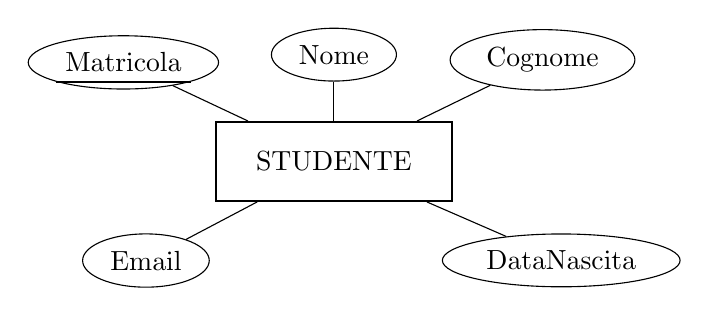
\begin{tikzpicture}[scale=0.75]
					% Entità Studente
					\node[rectangle, draw, thick, minimum width=3cm, minimum height=1cm] (studente) {STUDENTE};
					\node[ellipse, draw, above left=0.5cm and 0.3cm of studente] (matricola) {Matricola};
					\node[ellipse, draw, above=0.5cm of studente] (nome) {Nome};
					\node[ellipse, draw, above right=0.5cm and 0.3cm of studente] (cognome) {Cognome};
					\node[ellipse, draw, below left=0.5cm and 0.3cm of studente] (email) {Email};
					\node[ellipse, draw, below right=0.5cm and 0.3cm of studente] (data) {DataNascita};
					
					\draw (studente) -- (matricola);
					\draw (studente) -- (nome);
					\draw (studente) -- (cognome);
					\draw (studente) -- (email);
					\draw (studente) -- (data);
					
					% Sottolinea la chiave
					\draw[thick] (matricola.south west) -- (matricola.south east);
				\end{tikzpicture}
			\end{center}
		\end{columns}
	\end{frame}
	
	% Slide 17: Scegliere correttamente i nomi
	\begin{frame}{Scegliere correttamente i nomi}
		\begin{itemize}
			\item I nomi degli oggetti devono essere \textbf{unici}
			
			\item Devono avere un \textbf{significato} per l'utente finale
			
			\item Devono contenere il \textbf{numero minimo di parole} di cui si ha bisogno per descrivere univocamente e accuratamente l'oggetto
		\end{itemize}
	\end{frame}
	
	% Slide 18: Entità deboli e forti
	\begin{frame}{Entità deboli e forti}
		\begin{columns}
			\column{0.5\textwidth}
			Le entità che possiedono un insieme di attributi che le caratterizzano e hanno una \textbf{chiave primaria} prendono il nome di \textbf{entità forti}.
			
			\vspace{0.3cm}
			Esistono entità che non possiedono un proprio insieme di attributi che le identificano univocamente: tali entità si dicono \textbf{entità deboli}.
			
			\column{0.5\textwidth}
			\begin{center}
				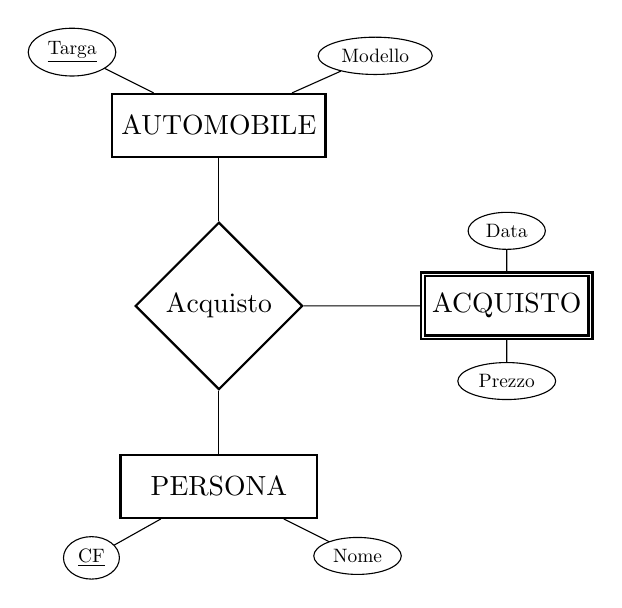
\begin{tikzpicture}[scale=0.7]
					% Entità forte: Automobile
					\node[rectangle, draw, thick, minimum width=2.5cm, minimum height=0.8cm] (auto) {AUTOMOBILE};
					\node[ellipse, draw, above left=0.3cm and 0.1cm of auto, scale=0.7] (targa) {\underline{Targa}};
					\node[ellipse, draw, above right=0.3cm and 0.1cm of auto, scale=0.7] (modello) {Modello};
					
					% Relazione
					\node[diamond, draw, thick, below=0.8cm of auto, minimum width=1cm] (rel) {Acquisto};
					
					% Entità forte: Persona
					\node[rectangle, draw, thick, below=0.8cm of rel, minimum width=2.5cm, minimum height=0.8cm] (persona) {PERSONA};
					\node[ellipse, draw, below left=0.3cm and 0.1cm of persona, scale=0.7] (cf) {\underline{CF}};
					\node[ellipse, draw, below right=0.3cm and 0.1cm of persona, scale=0.7] (nome) {Nome};
					
					% Entità debole: Acquisto
					\node[rectangle, draw, double, thick, right=1.5cm of rel, minimum width=2cm, minimum height=0.8cm] (acq) {ACQUISTO};
					\node[ellipse, draw, above=0.3cm of acq, scale=0.7] (data) {Data};
					\node[ellipse, draw, below=0.3cm of acq, scale=0.7] (prezzo) {Prezzo};
					
					\draw (auto) -- (targa);
					\draw (auto) -- (modello);
					\draw (persona) -- (cf);
					\draw (persona) -- (nome);
					\draw (acq) -- (data);
					\draw (acq) -- (prezzo);
					
					\draw (auto) -- (rel);
					\draw (rel) -- (persona);
					\draw (rel) -- (acq);
				\end{tikzpicture}
			\end{center}
		\end{columns}
	\end{frame}
	
	% Slide 19: Chiavi composte
	\begin{frame}{Chiavi composte}
		Quando nessun attributo singolo può fungere da chiave primaria, è possibile utilizzare una \textbf{chiave composta}.
		
		\vspace{0.5cm}
		\textbf{Esempio:} La coppia di attributi (DataAcquisto, Targa) identifica univocamente ogni singolo acquisto e la chiave primaria di Acquisto è una chiave composta, formata dalla coppia di chiavi parziali DataAcquisto e Targa (PPK, Partial Primary Key).
		
		\vspace{0.5cm}
		\textbf{Alternativa:} Per evitare di avere entità deboli si può aggiungere un attributo di tipo \textbf{numero progressivo} assegnato automaticamente, che identifica un'istanza dell'entità.
	\end{frame}
	
	% Slide 20: Molteplicità delle relazioni
	\begin{frame}{Molteplicità delle relazioni}
		La \textbf{molteplicità} di un'associazione è il numero di possibili istanze di un'entità, messo in corrispondenza con un'istanza dell'altra entità che partecipa all'associazione.
		
		\vspace{0.3cm}
		Il numero minimo e massimo di possibili istanze viene rappresentato mediante una coppia di valori separati da punti: \texttt{1..1}, \texttt{0..1}, \texttt{1..N}.
		
		\vspace{0.3cm}
		Al valore minimo e massimo sono associati gli importanti concetti di \textbf{obbligatorietà} e \textbf{cardinalità} dell'associazione:
		\begin{itemize}
			\item il valore minimo assume, in genere, uno dei due valori 0 e 1
			\begin{itemize}
				\item 0 indica che la partecipazione è \textbf{facoltativa}
				\item 1 indica che la partecipazione è \textbf{obbligatoria}
			\end{itemize}
			\item il valore massimo definisce la \textbf{cardinalità} della partecipazione all'associazione (1 oppure N)
		\end{itemize}
	\end{frame}
	
	% Slide 21: Le relazioni di tipo 1:1
	\begin{frame}{Le relazioni di tipo uno a uno (1:1)}
		\begin{columns}
			\column{0.5\textwidth}
			\textbf{Esempio:} Nazione - Capitale
			
			\vspace{0.3cm}
			\begin{itemize}
				\item Nazione ha come capitale una sola città (1 $\rightarrow$ 1)
				\begin{itemize}
					\item partecipazione obbligatoria
					\item molteplicità 1
				\end{itemize}
				
				\vspace{0.2cm}
				\item Un capitale appartiene ad una sola nazione (1 $\leftarrow$ 1)
				\begin{itemize}
					\item partecipazione obbligatoria
					\item molteplicità 1
				\end{itemize}
			\end{itemize}
			
			\column{0.5\textwidth}
			\begin{center}
				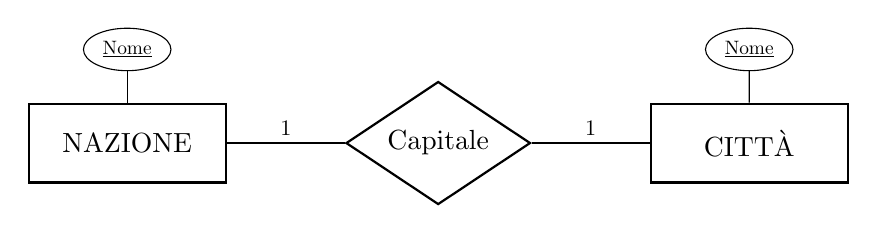
\begin{tikzpicture}[scale=0.8]
					% Entità Nazione
					\node[rectangle, draw, thick, minimum width=2.5cm, minimum height=1cm] (nazione) {NAZIONE};
					\node[ellipse, draw, above=0.4cm of nazione, scale=0.7] (nome1) {\underline{Nome}};
					
					% Relazione
					\node[diamond, draw, thick, right=1.5cm of nazione, minimum width=1cm, aspect=1.5] (capitale) {Capitale};
					
					% Entità Città
					\node[rectangle, draw, thick, right=1.5cm of capitale, minimum width=2.5cm, minimum height=1cm] (citta) {CITTÀ};
					\node[ellipse, draw, above=0.4cm of citta, scale=0.7] (nome2) {\underline{Nome}};
					
					% Connessioni
					\draw (nazione) -- (nome1);
					\draw (citta) -- (nome2);
					
					% Relazione con cardinalità
					\draw (nazione) -- node[above, scale=0.8] {1} (capitale);
					\draw (capitale) -- node[above, scale=0.8] {1} (citta);
				\end{tikzpicture}
			\end{center}
			
			\vspace{0.3cm}
			\small Ogni nazione ha esattamente una capitale, e ogni capitale appartiene a esattamente una nazione.
		\end{columns}
	\end{frame}
	
	% Slide 22: Relazioni uno a molti
	\begin{frame}{Relazioni uno a molti (1:N)}
		\begin{columns}
			\column{0.5\textwidth}
			Una relazione si dice \textbf{uno-a-molti} se esiste un'istanza della prima entità cui corrisponde più di un'istanza della seconda.
			
			\vspace{0.3cm}
			Viene anche indicata con \textbf{(1, n)}.
			
			\vspace{0.3cm}
			\textbf{Esempio:} 
			\begin{itemize}
				\item Una persona risiede in 1 città
				\item In una città risiedono N persone
			\end{itemize}
			
			\column{0.5\textwidth}
			\begin{center}
				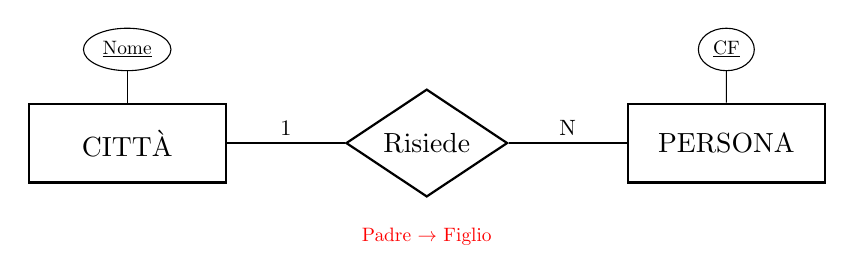
\begin{tikzpicture}[scale=0.8]
					% Entità Città
					\node[rectangle, draw, thick, minimum width=2.5cm, minimum height=1cm] (citta) {CITTÀ};
					\node[ellipse, draw, above=0.4cm of citta, scale=0.7] (nomec) {\underline{Nome}};
					
					% Relazione
					\node[diamond, draw, thick, right=1.5cm of citta, minimum width=1cm, aspect=1.5] (risiede) {Risiede};
					
					% Entità Persona
					\node[rectangle, draw, thick, right=1.5cm of risiede, minimum width=2.5cm, minimum height=1cm] (persona) {PERSONA};
					\node[ellipse, draw, above=0.4cm of persona, scale=0.7] (cf) {\underline{CF}};
					
					% Connessioni
					\draw (citta) -- (nomec);
					\draw (persona) -- (cf);
					
					% Relazione con cardinalità
					\draw (citta) -- node[above, scale=0.8] {1} (risiede);
					\draw (risiede) -- node[above, scale=0.8] {N} (persona);
					
					% Indicatore di direzione
					\node[below=0.3cm of risiede, scale=0.7, text=red] {Padre $\rightarrow$ Figlio};
				\end{tikzpicture}
			\end{center}
			
			\vspace{0.2cm}
			\small La città è l'entità "padre" nella relazione.
		\end{columns}
	\end{frame}
	
	% Slide 23: Relazioni molti a molti
	\begin{frame}{Relazioni di tipo molti a molti (N:M)}
		\begin{columns}
			\column{0.5\textwidth}
			Una relazione si dice \textbf{molti-a-molti} se esiste un'istanza della prima entità in relazione con più istanze della seconda, e viceversa.
			
			\vspace{0.3cm}
			Viene indicata con \textbf{(n, n)} o \textbf{(N, M)}.
			
			\vspace{0.3cm}
			\textbf{Esempio:} 
			\begin{itemize}
				\item Uno studente frequenta più corsi
				\item Un corso è frequentato da più studenti
			\end{itemize}
			
			\column{0.5\textwidth}
			\begin{center}
				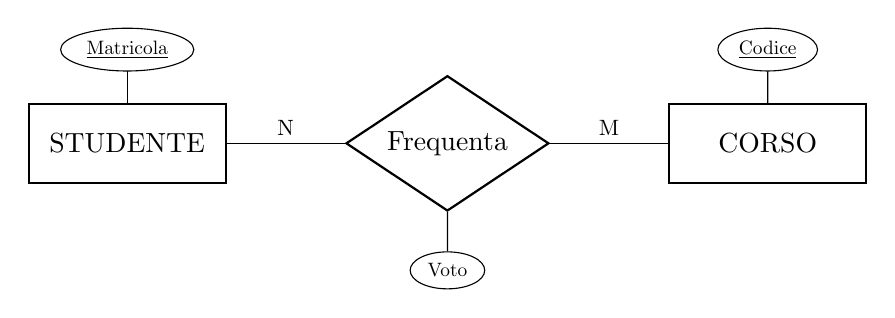
\begin{tikzpicture}[scale=0.75]
					% Entità Studente
					\node[rectangle, draw, thick, minimum width=2.5cm, minimum height=1cm] (studente) {STUDENTE};
					\node[ellipse, draw, above=0.4cm of studente, scale=0.7] (matr) {\underline{Matricola}};
					
					% Relazione
					\node[diamond, draw, thick, right=1.5cm of studente, minimum width=1cm, aspect=1.5] (freq) {Frequenta};
					
					% Entità Corso
					\node[rectangle, draw, thick, right=1.5cm of freq, minimum width=2.5cm, minimum height=1cm] (corso) {CORSO};
					\node[ellipse, draw, above=0.4cm of corso, scale=0.7] (cod) {\underline{Codice}};
					
					% Attributo della relazione
					\node[ellipse, draw, below=0.5cm of freq, scale=0.7] (voto) {Voto};
					
					% Connessioni
					\draw (studente) -- (matr);
					\draw (corso) -- (cod);
					\draw (freq) -- (voto);
					
					% Relazione con cardinalità
					\draw (studente) -- node[above, scale=0.8] {N} (freq);
					\draw (freq) -- node[above, scale=0.8] {M} (corso);
				\end{tikzpicture}
			\end{center}
			
			\vspace{0.2cm}
			\small La relazione può avere attributi propri (es. Voto).
		\end{columns}
	\end{frame}
	
	% Slide 24: Esistenza obbligatoria e opzionale
	\begin{frame}{Esistenza obbligatoria e opzionale}
		\begin{columns}
			\column{0.5\textwidth}
			\textbf{Esistenza obbligatoria:}
			\begin{itemize}
				\item Un'istanza deve partecipare alla relazione
				\item Valore minimo = 1
			\end{itemize}
			
			\vspace{0.3cm}
			\textbf{Esistenza opzionale:}
			\begin{itemize}
				\item Partecipazione facoltativa
				\item Valore minimo = 0
			\end{itemize}
			
			\vspace{0.3cm}
			\small Nel caso di relazione (1,1) il numero può essere omesso.
			
			\column{0.5\textwidth}
			\begin{center}
				\textbf{Esempio: Prestito libri}
				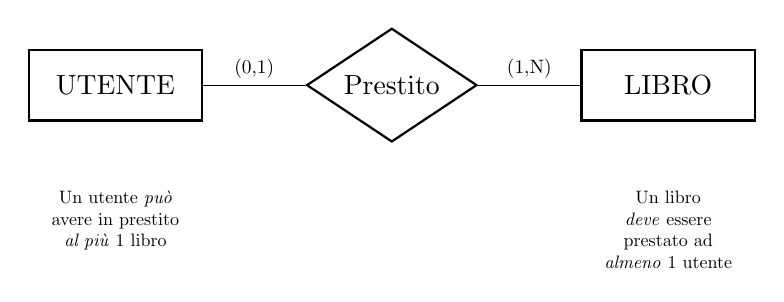
\begin{tikzpicture}[scale=0.7]
					% Entità Utente
					\node[rectangle, draw, thick, minimum width=2.2cm, minimum height=0.9cm] (utente) {UTENTE};
					
					% Relazione
					\node[diamond, draw, thick, right=1.3cm of utente, minimum width=0.8cm, aspect=1.5] (prestito) {Prestito};
					
					% Entità Libro
					\node[rectangle, draw, thick, right=1.3cm of prestito, minimum width=2.2cm, minimum height=0.9cm] (libro) {LIBRO};
					
					% Connessioni con cardinalità
					\draw (utente) -- node[above, scale=0.7] {(0,1)} (prestito);
					\draw (prestito) -- node[above, scale=0.7] {(1,N)} (libro);
					
					% Annotazioni
					\node[below=0.8cm of utente, text width=2.5cm, align=center, scale=0.65] {Un utente \textit{può} avere in prestito \textit{al più} 1 libro};
					\node[below=0.8cm of libro, text width=2.5cm, align=center, scale=0.65] {Un libro \textit{deve} essere prestato ad \textit{almeno} 1 utente};
				\end{tikzpicture}
			\end{center}
		\end{columns}
	\end{frame}
	
	% Slide 25: Direzione della relazione
	\begin{frame}{Direzione della relazione}
		Riconsiderando l'esempio delle entità \textit{studente} e \textit{città}, si vede che, poiché la relazione tra città e studente ha cardinalità uno-a-molti, la direzione è \textbf{da città a studente} $\rightarrow$
		
		\vspace{0.5cm}
		L'entità \textit{città} è \textbf{padre} rispetto all'entità \textit{studente}.
		
		\vspace{0.5cm}
		La direzione della relazione indica qual è l'entità da cui parte la relazione verso l'altra entità.
	\end{frame}
	
	% Slide 26: Relazione gerarchica
	\begin{frame}{Relazione gerarchica tra entità}
		\begin{columns}
			\column{0.5\textwidth}
			Esistono situazioni in cui tra le entità può essere stabilita una \textbf{gerarchia}, come nella programmazione OOP.
			
			\vspace{0.3cm}
			\begin{itemize}
				\item \textbf{beta} è detta \textit{sottoclasse} o \textit{specializzazione}
				\item \textbf{alfa} è detta \textit{superclasse} o \textit{generalizzazione}
			\end{itemize}
			
			\vspace{0.3cm}
			\textbf{Due vincoli:}
			\begin{enumerate}
				\item \textbf{Struttura}: ereditarietà di attributi e associazioni
				\item \textbf{Insieme}: beta $\subseteq$ alfa
			\end{enumerate}
			
			\column{0.5\textwidth}
			\begin{center}
				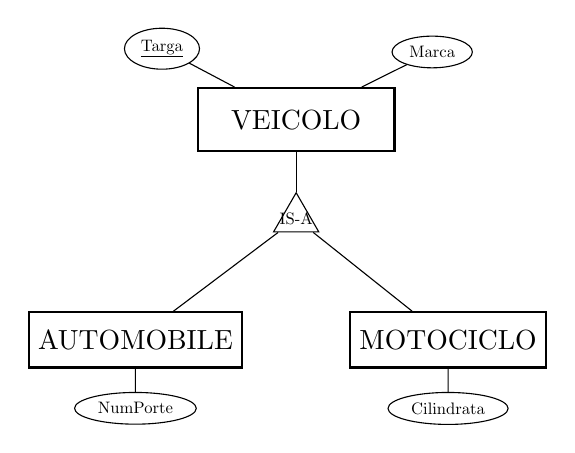
\begin{tikzpicture}[scale=0.75]
					% Superclasse
					\node[rectangle, draw, thick, minimum width=2.5cm, minimum height=0.8cm] (veicolo) {VEICOLO};
					\node[ellipse, draw, above left=0.3cm and 0.1cm of veicolo, scale=0.6] (targa) {\underline{Targa}};
					\node[ellipse, draw, above right=0.3cm and 0.1cm of veicolo, scale=0.6] (marca) {Marca};
					
					% Simbolo generalizzazione
					\node[draw, regular polygon, regular polygon sides=3, minimum size=0.6cm, below=0.5cm of veicolo] (gen) {};
					\node[scale=0.6] at (gen) {IS-A};
					
					% Sottoclassi
					\node[rectangle, draw, thick, below left=1cm and 0.5cm of gen, minimum width=2cm, minimum height=0.7cm] (auto) {AUTOMOBILE};
					\node[ellipse, draw, below=0.3cm of auto, scale=0.6] (porte) {NumPorte};
					
					\node[rectangle, draw, thick, below right=1cm and 0.5cm of gen, minimum width=2cm, minimum height=0.7cm] (moto) {MOTOCICLO};
					\node[ellipse, draw, below=0.3cm of moto, scale=0.6] (cilindrata) {Cilindrata};
					
					% Connessioni
					\draw (veicolo) -- (targa);
					\draw (veicolo) -- (marca);
					\draw (veicolo) -- (gen);
					\draw (gen) -- (auto);
					\draw (gen) -- (moto);
					\draw (auto) -- (porte);
					\draw (moto) -- (cilindrata);
				\end{tikzpicture}
			\end{center}
		\end{columns}
	\end{frame}
	
	% Slide 27: Copertura delle generalizzazioni
	\begin{frame}{Copertura delle generalizzazioni}
		\begin{columns}
			\column{0.55\textwidth}
			Le generalizzazioni si caratterizzano per "due dimensioni indipendenti":
			
			\vspace{0.2cm}
			\textbf{1. Unione vs classe generalizzata:}
			\begin{itemize}
				\item \textbf{Totale}: unione = generalizzata
				\item \textbf{Parziale}: unione $\subset$ generalizzata
			\end{itemize}
			
			\vspace{0.2cm}
			\textbf{2. Confronto fra specializzate:}
			\begin{itemize}
				\item \textbf{Esclusiva}: disgiunte
				\item \textbf{Sovrapposta}: intersezione $\neq \emptyset$
			\end{itemize}
			
			\column{0.45\textwidth}
			\begin{center}
				\textbf{Esempio: Totale ed Esclusiva}
				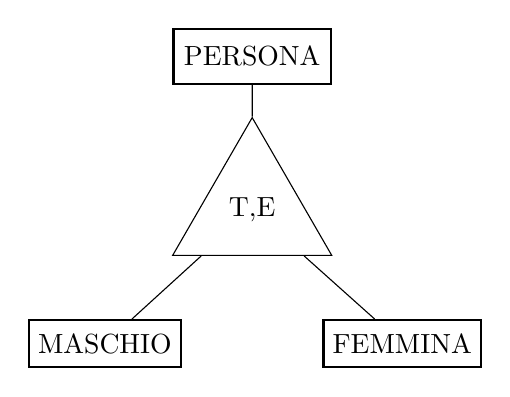
\begin{tikzpicture}[scale=0.6]
					\node[rectangle, draw, thick, minimum width=2cm, minimum height=0.7cm] (persona) {PERSONA};
					\node[draw, regular polygon, regular polygon sides=3, minimum size=0.5cm, below=0.4cm of persona] (gen1) {T,E};
					
					\node[rectangle, draw, thick, below left=0.8cm and 0.3cm of gen1, minimum width=1.5cm, minimum height=0.6cm] (m) {MASCHIO};
					\node[rectangle, draw, thick, below right=0.8cm and 0.3cm of gen1, minimum width=1.5cm, minimum height=0.6cm] (f) {FEMMINA};
					
					\draw (persona) -- (gen1);
					\draw (gen1) -- (m);
					\draw (gen1) -- (f);
				\end{tikzpicture}
				
				\vspace{0.3cm}
				\textbf{Esempio: Parziale e Sovrapposta}
				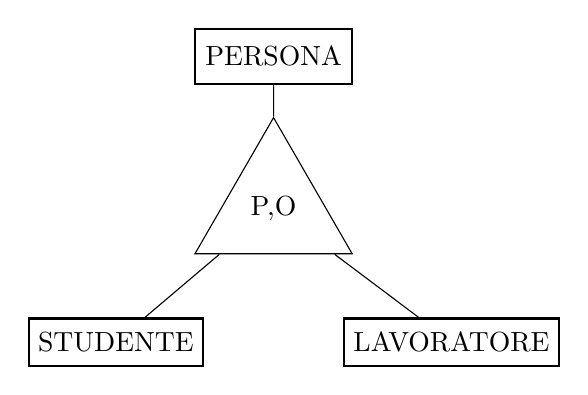
\begin{tikzpicture}[scale=0.6]
					\node[rectangle, draw, thick, minimum width=2cm, minimum height=0.7cm] (persona2) {PERSONA};
					\node[draw, regular polygon, regular polygon sides=3, minimum size=0.5cm, below=0.4cm of persona2] (gen2) {P,O};
					
					\node[rectangle, draw, thick, below left=0.8cm and 0.3cm of gen2, minimum width=1.5cm, minimum height=0.6cm] (st) {STUDENTE};
					\node[rectangle, draw, thick, below right=0.8cm and 0.3cm of gen2, minimum width=1.5cm, minimum height=0.6cm] (lav) {LAVORATORE};
					
					\draw (persona2) -- (gen2);
					\draw (gen2) -- (st);
					\draw (gen2) -- (lav);
				\end{tikzpicture}
			\end{center}
		\end{columns}
	\end{frame}
	
	% Slide 28: Esempio completo di diagramma E-R
	\begin{frame}{Esempio completo: Sistema Biblioteca}
		\begin{center}
			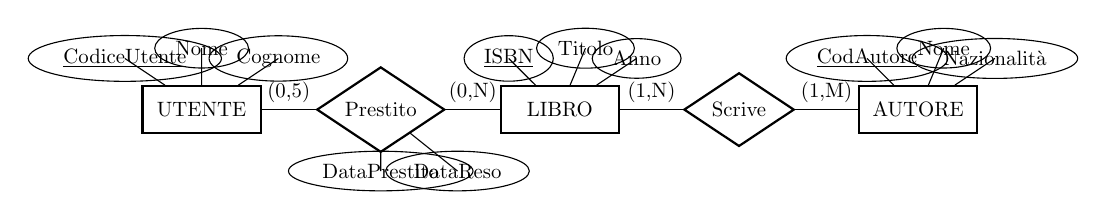
\begin{tikzpicture}[scale=0.65, every node/.style={scale=0.75}]
				% Entità UTENTE
				\node[rectangle, draw, thick, minimum width=2cm, minimum height=0.8cm] (utente) at (0,0) {UTENTE};
				\node[ellipse, draw] at (-1.5,1) {\underline{CodiceUtente}};
				\node[ellipse, draw] at (0,1.2) {Nome};
				\node[ellipse, draw] at (1.5,1) {Cognome};
				\draw (utente) -- (-1.5,1);
				\draw (utente) -- (0,1.2);
				\draw (utente) -- (1.5,1);
				
				% Relazione PRESTITO
				\node[diamond, draw, thick, minimum width=1cm, aspect=1.5] (prestito) at (3.5,0) {Prestito};
				\node[ellipse, draw] at (3.5,-1.2) {DataPrestito};
				\node[ellipse, draw] at (5,-1.2) {DataReso};
				\draw (prestito) -- (3.5,-1.2);
				\draw (prestito) -- (5,-1.2);
				
				% Entità LIBRO
				\node[rectangle, draw, thick, minimum width=2cm, minimum height=0.8cm] (libro) at (7,0) {LIBRO};
				\node[ellipse, draw] at (6,1) {\underline{ISBN}};
				\node[ellipse, draw] at (7.5,1.2) {Titolo};
				\node[ellipse, draw] at (8.5,1) {Anno};
				\draw (libro) -- (6,1);
				\draw (libro) -- (7.5,1.2);
				\draw (libro) -- (8.5,1);
				
				% Relazione SCRIVE
				\node[diamond, draw, thick, minimum width=1cm, aspect=1.5] (scrive) at (10.5,0) {Scrive};
				
				% Entità AUTORE
				\node[rectangle, draw, thick, minimum width=2cm, minimum height=0.8cm] (autore) at (14,0) {AUTORE};
				\node[ellipse, draw] at (13,1) {\underline{CodAutore}};
				\node[ellipse, draw] at (14.5,1.2) {Nome};
				\node[ellipse, draw] at (15.5,1) {Nazionalità};
				\draw (autore) -- (13,1);
				\draw (autore) -- (14.5,1.2);
				\draw (autore) -- (15.5,1);
				
				% Connessioni e cardinalità
				\draw (utente) -- node[above] {(0,5)} (prestito);
				\draw (prestito) -- node[above] {(0,N)} (libro);
				\draw (libro) -- node[above] {(1,N)} (scrive);
				\draw (scrive) -- node[above] {(1,M)} (autore);
			\end{tikzpicture}
		\end{center}
		
		\vspace{0.2cm}
		\small\textbf{Legenda:} Un utente può avere fino a 5 prestiti, un libro può essere prestato a più utenti, un libro ha almeno un autore, un autore scrive più libri.
	\end{frame}
	
	% Slide finale
	\begin{frame}
		\begin{center}
			{\Huge Grazie per l'attenzione!}
			
			\vspace{1cm}
			{\large Domande?}
		\end{center}
	\end{frame}
	
\end{document}